\section{Experimenty}

Experimenty této práce probíhaly především na počítačích uvedených v předchozí kapitole. Nejprve je však vhodné zmínit konfiguraci daných počítačů:
\begin{itemize}
\item\textbf{HummingBoard Pro} - na tomto počítači je nainstalován Linux Debian 8.1 s označením ``jessie'' s grafickým rozhraním MATE 8.
\item\textbf{Banana PI} - na tomto počítači je nainstalován Linux Debian 8.1 s označením ``jessie'' s grafickým rozhraním Xfce 4.10. 
\item\textbf{Raspberry PI} - na tomto počítači je nainstalován Linux Raspbian. 
\end{itemize}
Dále pro srovnání výkonu těchto počítačů byl program otestován i na desktopovém počítači, na kterém byl i vyvíjen a odladěn. Jeho konfigurace zní: 
\begin{itemize}
\item\textit{Intel Core i7-6700k}, operační paměť  \textit{32 GB} a operační systém  \textit{Windows 10 Pro}.
\end{itemize}
Prvním sada experimentů byla detekce pomocí histogramů orientovaných hran a jeho vylepšení pomocí algoritmu pro substrakci pozadí při detekci ze statických kamer.

\subsection{Nalezení optimálního klasifikátoru}

Nalezení optimálního a spolehlivého klasifikátoru je klíčovou částí celého procesu, zároveň se jedná i o velmi komplikovaný a zdlouhavý úkol. Je důležité zvolit ideální tréninkovou sadu vzorků a k vzhledem zvoleného typu SVM a jejího jádra. Otestoval jsem varianty $C$, $\nu$, $\varepsilon$-SVR klasifikátorové typy s lineárním a Gaussovým jádrem, přičemž jsem zjistil, že nejlepší sestava pro detekování chodců je kombinace typu $\varepsilon$-SVR s lineárním jádrem, protože pozitivní detekce byla poměrně větší než negativní. Při zvolení správného jádra a typu klasifikátoru je dalším krokem vybrat, jak už bylo zmíněno, tréninkovou sadu. Vyzkoušel jsem nejrůznější tréninkové sady dostupné na internetu a jejich kombinace.

Nejlepších výsledků jsem dosáhl s pozitivní trénovací sadou pana Dase \cite{sudipdas}, CUHK01 campus \cite{cuhk} a jako negativní sadu jsem použil Daimler-Mono\cite{daimler}, kterou jsem nastříhal na vzorky. Tyto sady jsou přiloženy v příloze této práce. Následujícím krokem je zvolení správných parametrů trénování klasifikátoru. 

Trénování klasifikátoru je velmi citlivé na tyto parametry, při změně některého z nich jen o tisícinu, můžeme získat úplně jiný výsledek. Trénování probíhalo dvakrát za sebou. Při druhém trénování se klasifikátor učil ze svých špatných detekcí, čemuž se říká ``Bootstrapping''. To znamená, že detekce se spustila na negativních vzorcích s tímto klasifikátorem a pokud detektor vrátil nějaký výsledek, byl zpět uložen do negativní sady a znovu natrénován, tento postup je ilustrován ve zdrojovém kódu \ref{src:double_train}.
\newpage

\begin{lstlisting}[label=src:double_train, language=cpp, caption=Bootstrapping]
		cv::Size posSize = posSamplesLst[0].size();
		cv::HOGDescriptor myHog;
		myHog.winSize = posSize;
		std::vector < cv::Rect > locations;
		std::vector < float > hogDetector;
		
		getSvmDetector(svm, hogDetector);
		myHog.setSVMDetector(hogDetector);

		std::vector < cv::Rect > detections;

		for (size_t i = 0; i < negSamplesLst.size(); i++)	{
			myHog.detectMultiScale(negSamplesLst[i], detections);
			for (size_t j = 0; j < detections.size(); j++)	{
				cv::Mat detection = negSamplesLst[i](detections[j]).clone();
				resize(detection, detection, posSize);
				negSamplesLst.push_back(detection);
			}
		}
		labels.clear();
		labels.assign(posSamplesLst.size(), +1);
		labels.insert(labels.end(), negSamplesLst.size(), 0);

		gradientLst.clear();
		extractFeatures(posSamplesLst, gradientLst);
		extractFeatures(negSamplesLst, gradientLst);

		convertSamples2Mat(gradientLst, trainMat);
		trainSvm(trainMat, labels);
\end{lstlisting}

Natrénoval jsem klasifikátory s různými parametry a otestoval je na testovacích vzorcích. Tyto vzorky byly vyextrahované obrázky chodců a "ne-chodců" z testovacích videí pomocí jejich anotací a přiloženého nástroje pro tvorbu vzorků a také z projektu PETA, konkrétně se jednalo o sady: \textit{3DPeS, CAVIAR4REID, CBLC, SARC3D, VIPeR}. Tento krok je v podstatě první filtrací klasifikátorů, aby detekoval, co nejvíce chodců a nedetekoval oblasti, kde nejsou. Vytrénoval jsem 15 klasifikátorů s různými parametry trénování. Tyto klasifikátory jsem nadále filtroval pomocí ROC křivky a vizuálně vybral ten nejlepší z obrázku \ref{fig:rocCurve1}.  Nastavení trénovacích parametrů jsou uvedeny v tabulce \ref{classTab1}.  

\begin{figure}[H]
\centering
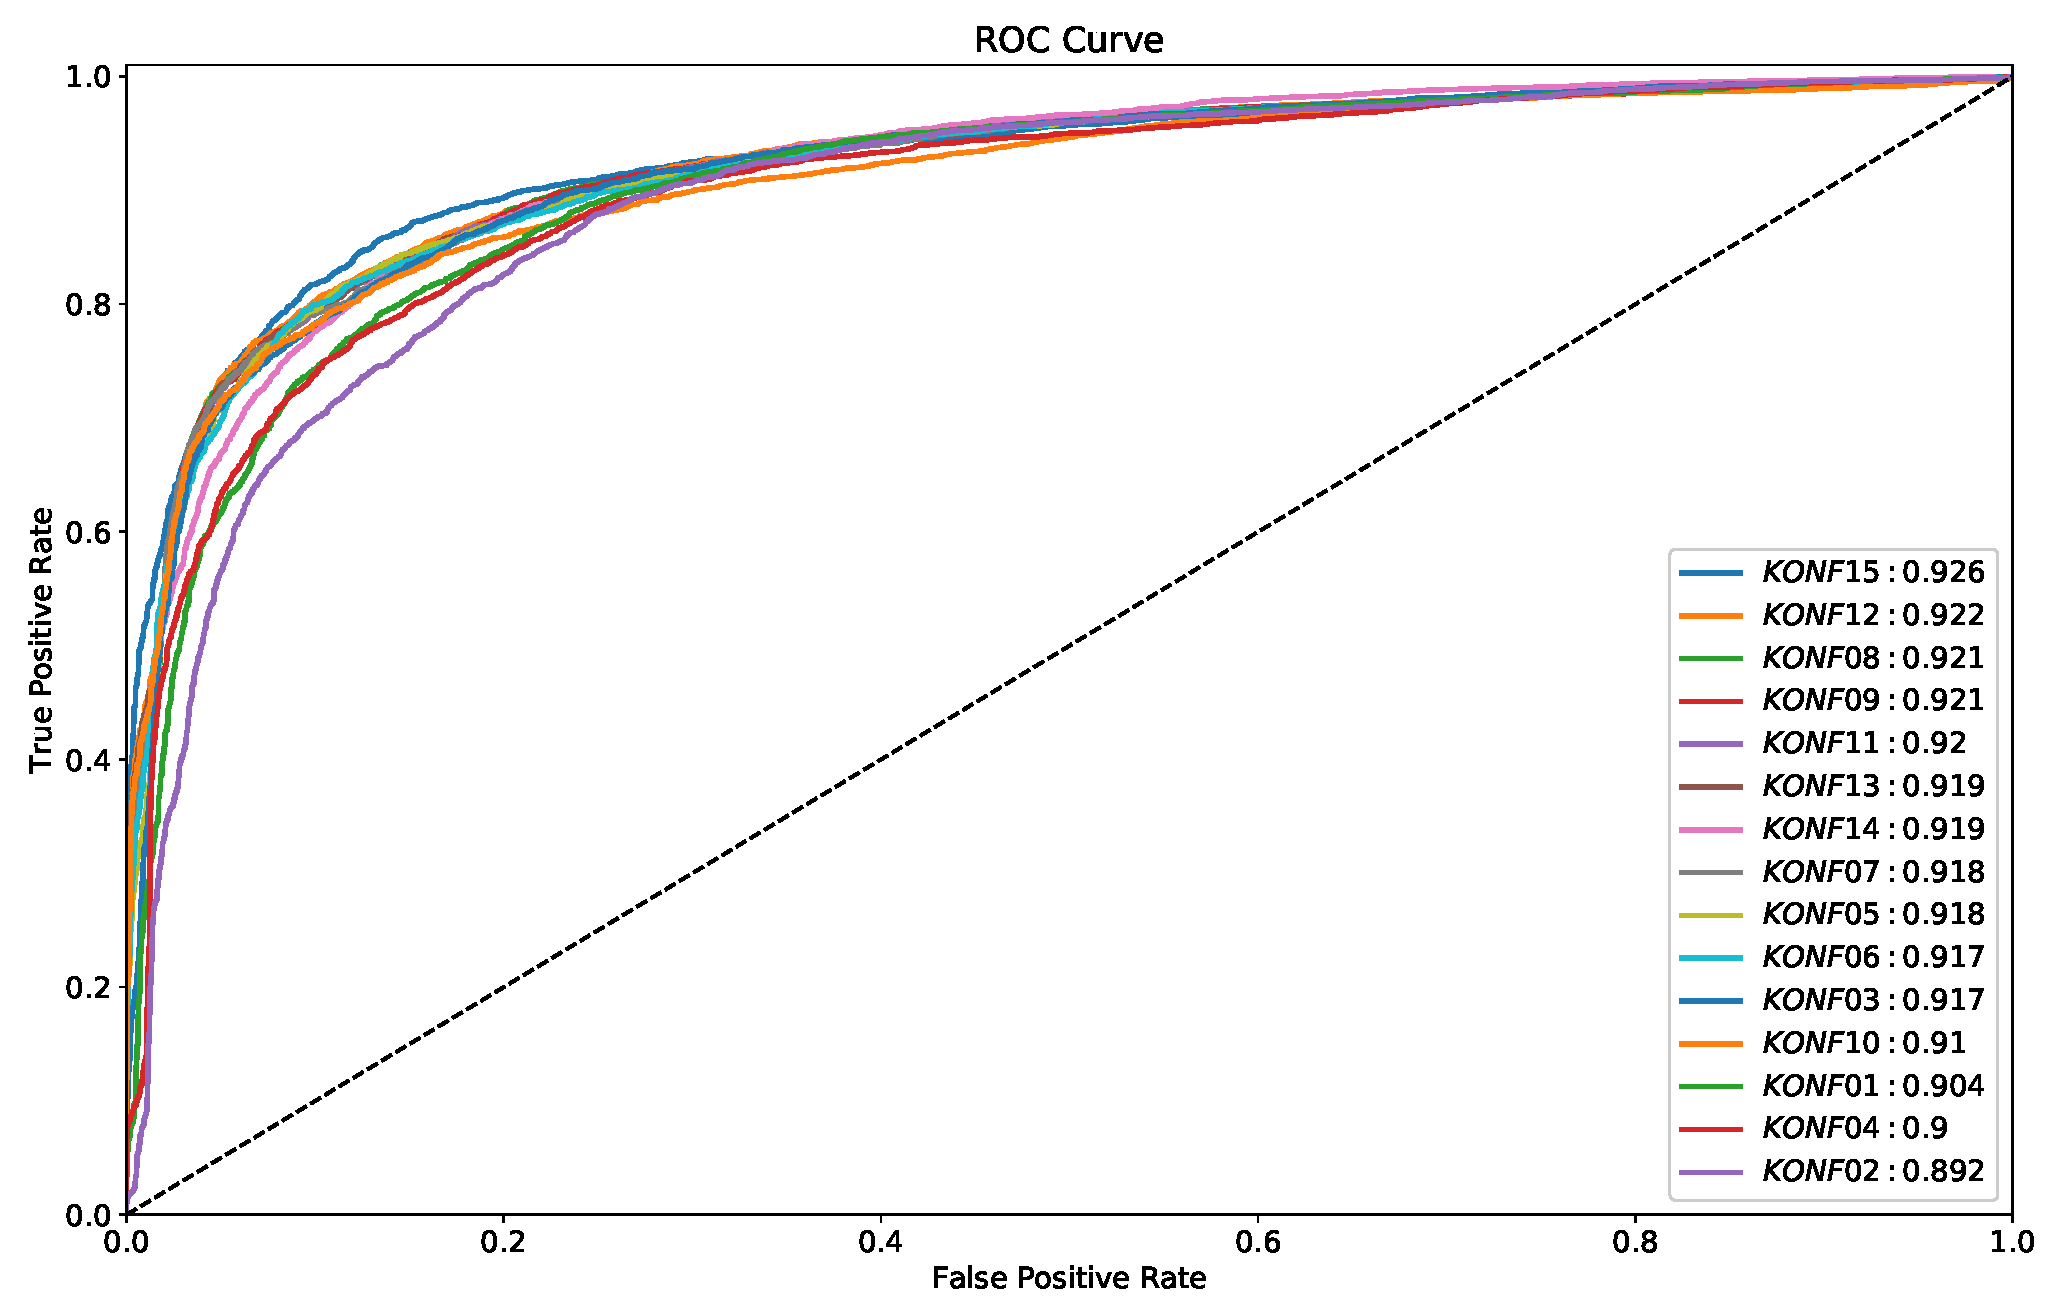
\includegraphics[width=16cm]{figures/roc1}
\caption{ROC křivka natrénovaných klasifikátorů}
\label{fig:rocCurve1}
\end{figure}

\begin{table}[H]
\centering
\caption{Přehled vytrénovaných klasifikátorů a jejich trénovacích parametrů. Parametry $\varepsilon$, kritéria ukončení a počet pozitivních vzorků (5649) byly stejné.}
\begin{tabular} { |c|c|c|c|c|c| }
\hline
{}          & {par. C} & {par. P}    & {max iterací} & {počet neg. vzorků} & {Přesnost \%}  \\ \hline
KONF 01		& 	0.005	& 	  0.02	 &   2000   	 &		  3000   	   &     83	 		\\ \hline
KONF 02		& 	0.005	& 	  0.01	 &   3500   	 &		  3000   	   &     81	 		\\ \hline
KONF 03		& 	0.001	& 	  0.02	 &   2000   	 &		  6000   	   &     83	 		\\ \hline
KONF 04		& 	0.001	& 	  0.02	 &   4500   	 &		  6000   	   &     81	 		\\ \hline
KONF 05		& 	0.005	& 	  0.4 	 &   3500   	 &		  6000   	   &     84	 		\\ \hline
KONF 06		& 	0.01 	& 	  0.4 	 &   3000   	 &		  6000   	   &     84	 		\\ \hline
KONF 07		& 	0.005	& 	  0.01	 &   2500   	 &		  9000   	   &     82	 		\\ \hline
KONF 08		& 	0.005	& 	  0.25	 &   2000   	 &		  9000   	   &     82	 		\\ \hline
KONF 09		& 	0.005	& 	  0.25	 &   3000   	 &		  9000   	   &     82	 		\\ \hline
KONF 10 	& 	0.01 	& 	  0.02	 &   3000   	 &		  9000   	   &     80	 		\\ \hline
KONF 11 	& 	0.01 	& 	  0.25	 &   2000   	 &		  9000   	   &     82	 		\\ \hline
KONF 12 	& 	0.01 	& 	  0.25	 &   2500   	 &		  9000   	   &     82	 		\\ \hline
KONF 13 	& 	0.01 	& 	  0.25	 &   4500   	 &		  9000   	   &     82	 		\\ \hline
KONF 14 	& 	0.5	 	& 	  0.1	 &   1200   	 &		  9000   	   &     81	 		\\ \hline
KONF 15 	& 	0.5		& 	  0.1	 &   2000   	 &		  9000   	   &     83	 		\\ \hline
\end{tabular}
\label{classTab1}
\end{table}

Vybral jsem konfiguraci 15, protože oblast pod křivkou byla největší ze všech natrénovaných, přesnost tohoto klasifikátoru je v tabulce \ref{classTab2}. Výsledky testování ostatních klasifikátorů jsou v příloze této práce. Detekce může nabývat maximálně 4 stavů:
\begin{itemize}
	\item{True Positive (\textbf{TP}) - detektor správně rozpoznal chodce.}
	\item{True Negative (\textbf{TN}) - detektor tuto oblast ignoroval.}
	\item{False Positive (\textbf{FP}) - detektor označil tuto oblast za chodce, ovšem se zde nenachází.}
	\item{False Negative (\textbf{FN}) - v oblasti se vyskytuje chodec avšak byl ignorován.}
\end{itemize}

Díky těmto stavům můžeme vypočítat přesnost detekce:
\begin{equation*}
\centering
 \label{eq:accuracy}
 \begin{aligned}
Accuracy = \frac{TP + TN}{TP + TN + FP + FN}
 \end{aligned}
\end{equation*}

\begin{table}[H]
\centering
\caption{Přesnost konfigurace klasifikátoru číslo}
\begin{tabular} { |c|c|c|c|c| }
\hline
{}          & {TP/FN} 	 & {TN/FP} 	& {Přesnost \%} & {AUC}  \\ \hline
KONF 15 	&  3479/1572 & 4912/192 &     83 		& 0.926  \\ \hline
\end{tabular}
\label{classTab2}
\end{table}
Na tento klasifikátor jsem se rozhodl aplikovat algoritmus substrakce pozadí a tak zefektivnit jeho rychlost a správnost detekce.

\subsection{Aplikace algoritmu Mixtura Gaussiánů}
V předchozí kapitole jsem popsal, jak probíhalo zvolení optimálního klasifikátoru a nyní jej pojďme použít na reálná data. Chodci jsou v použitých videosekvencích a obrázcích anotováni v textových souborech každý zvlášť. První řádek tohoto textového souboru odpovídá počtu snímku videa a další řádky jsou věnovány samotným anotacím, kde první číslo vyjadřuje číslo snímku a následující 4 čísla jsou body dané anotace.

Testovací video je ve 3 druzích rozlišení, základní informace o videosekvencích je uvedena v tabulce \ref{videosTab}, rozdíl mezi výskytem osob a snímků za sekundu je způsobené převodem videa.

\begin{table}[H]
\centering
\caption{Přehled testovaných videozáznamů}
\begin{tabular} { |c|c|c|c|c| }
\hline
{Název videa}   & {Rozlišení} 	& {Počet snímků}    & {FPS} & {Výskyt osob na snímcích}  	\\ \hline
cctv4.mp4 		&  640 x  360	& 781  				& 29,97	& 	754				\\ \hline
cctv4.avi		& 1280 x  720	& 626  				& 24,00	& 	597				\\ \hline
cctv4.mov 		& 1920 x 1080	& 781  				& 29,97	& 	749				\\ \hline
\end{tabular}
\label{videosTab}
\end{table}

Chodci se ve videosekvenci mohli vyskytovat kdekoliv, proto jsem namísto přesnosti, počítal F1-skóre, které taky vyjadřuje, ale ke svému výpočtu nepotřebuje true negative, které by bylo nemožné získat z každého obrázku z videa. Výpočet F1-skóre je následující:
\begin{equation*}
\centering
 \label{eq:f1score}
 \begin{aligned}
F1-score = \frac{ 2TP}{2TP + FP + FN}
 \end{aligned}
\end{equation*}
Také jsem stanovil pravidlo pro pozitivní detekci a to takové, že výstup z detektoru je považován za pozitivní právě tehdy, když jeho plocha je větší než polovina anotované plochy.
V následujících tabulkách jsou uvedeny výsledek detekce z každého videa na každém zařízení. \ref{resultTabIMX} \ref{resultTabRPI3} \ref{resultTabBPI}.
\begin{table}[H]
\catcode`\-=12
\centering
\caption{Výsledky detekce počítače HummingBoard Pro i.MX6 }
\label{resultTabIMX}
\begin{tabular}{|c|l|l|l|l|l|l|l|}
\hline
                         & Typ algoritmu   	& ALG FPS & Délka detekce & TP & FN & FP & F1-skóre \\ \hline
\multirow{4}{*}{cctv4.mp4} & HOG        	&         &               &    &    &    &          \\ \cline{2-8} 
                         & HOG + MOG  		&         &               &    &    &    &          \\ \cline{2-8} 
                         & FHOG       		&         &               &    &    &    &          \\ \cline{2-8} 
                         & FHOG + MOG 		&         &               &    &    &    &          \\ \hline\hline 
\multirow{4}{*}{cctv4.avi} & HOG        	&         &               &    &    &    &          \\ \cline{2-8} 
                         & HOG + MOG  		&         &               &    &    &    &          \\ \cline{2-8} 
                         & FHOG       		&         &               &    &    &    &          \\ \cline{2-8} 
                         & FHOG + MOG 		&         &               &    &    &    &          \\ \hline \hline
\multirow{4}{*}{cctv4.mov} & HOG        	&         &               &    &    &    &          \\ \cline{2-8} 
                         & HOG + MOG  		&         &               &    &    &    &          \\ \cline{2-8} 
                         & FHOG       		&         &               &    &    &    &          \\ \cline{2-8} 
                         & FHOG + MOG 		&         &               &    &    &    &          \\ \hline
\end{tabular}
\end{table}


\begin{table}[H]
\catcode`\-=12
\centering
\caption{Výsledky detekce počítače Raspberry PI3}
\label{resultTabRPI3}
\begin{tabular}{|c|l|l|l|l|l|l|l|}
\hline
                         & Typ algoritmu   & ALG FPS & Délka detekce & TP & FN & FP & F1-skóre \\ \hline
\multirow{4}{*}{cctv4.mp4} & HOG        &         &               &    &    &    &          \\ \cline{2-8} 
                         & HOG + MOG  &         &               &    &    &    &          \\ \cline{2-8} 
                         & FHOG       &         &               &    &    &    &          \\ \cline{2-8} 
                         & FHOG + MOG &         &               &    &    &    &          \\ \hline\hline 
\multirow{4}{*}{cctv4.avi} & HOG        &         &               &    &    &    &          \\ \cline{2-8} 
                         & HOG + MOG  &         &               &    &    &    &          \\ \cline{2-8} 
                         & FHOG       &         &               &    &    &    &          \\ \cline{2-8} 
                         & FHOG + MOG &         &               &    &    &    &          \\ \hline \hline
\multirow{4}{*}{cctv4.mov} & HOG        &         &               &    &    &    &          \\ \cline{2-8} 
                         & HOG + MOG  &         &               &    &    &    &          \\ \cline{2-8} 
                         & FHOG       &         &               &    &    &    &          \\ \cline{2-8} 
                         & FHOG + MOG &         &               &    &    &    &          \\ \hline
\end{tabular}
\end{table}


\begin{table}[H]
\catcode`\-=12
\centering
\caption{Výsledky detekce počítače Banana PI BPI-M1}
\label{resultTabBPI}
\begin{tabular}{|c|l|l|l|l|l|l|l|}
\hline
                         & Typ algoritmu   & ALG FPS & Délka detekce & TP & FN & FP & F1-skóre \\ \hline
\multirow{4}{*}{cctv4.mp4} & HOG        &         &               &    &    &    &          \\ \cline{2-8} 
                         & HOG + MOG  &         &               &    &    &    &          \\ \cline{2-8} 
                         & FHOG       &         &               &    &    &    &          \\ \cline{2-8} 
                         & FHOG + MOG &         &               &    &    &    &          \\ \hline\hline 
\multirow{4}{*}{cctv4.avi} & HOG        &         &               &    &    &    &          \\ \cline{2-8} 
                         & HOG + MOG  &         &               &    &    &    &          \\ \cline{2-8} 
                         & FHOG       &         &               &    &    &    &          \\ \cline{2-8} 
                         & FHOG + MOG &         &               &    &    &    &          \\ \hline \hline
\multirow{4}{*}{cctv4.mov} & HOG        &         &               &    &    &    &          \\ \cline{2-8} 
                         & HOG + MOG  &         &               &    &    &    &          \\ \cline{2-8} 
                         & FHOG       &         &               &    &    &    &          \\ \cline{2-8} 
                         & FHOG + MOG &         &               &    &    &    &          \\ \hline
\end{tabular}
\end{table}

\begin{table}[H]
\catcode`\-=12
\centering
\caption{Výsledky detekce desktopového počítače}
\label{resultTabDesktop}
\begin{tabular}{|c|l|l|l|l|l|l|l|}
\hline
                         & Typ algoritmu   & ALG FPS & Délka detekce & TP & FN & FP & F1-skóre \\ \hline
\multirow{4}{*}{cctv4.mp4} & HOG        &         &               &    &    &    &          \\ \cline{2-8} 
                         & HOG + MOG  &         &               &    &    &    &          \\ \cline{2-8} 
                         & FHOG       &         &               &    &    &    &          \\ \cline{2-8} 
                         & FHOG + MOG &         &               &    &    &    &          \\ \hline\hline 
\multirow{4}{*}{cctv4.avi} & HOG        &         &               &    &    &    &          \\ \cline{2-8} 
                         & HOG + MOG  &         &               &    &    &    &          \\ \cline{2-8} 
                         & FHOG       &         &               &    &    &    &          \\ \cline{2-8} 
                         & FHOG + MOG &         &               &    &    &    &          \\ \hline \hline
\multirow{4}{*}{cctv4.mov} & HOG        &         &               &    &    &    &          \\ \cline{2-8} 
                         & HOG + MOG  &         &               &    &    &    &          \\ \cline{2-8} 
                         & FHOG       &         &               &    &    &    &          \\ \cline{2-8} 
                         & FHOG + MOG &         &               &    &    &    &          \\ \hline
\end{tabular}
\end{table}
 První trénování --->špatný dataset
 druhé trénování --->špatné parametry
 třetí trénování --->téměř dobré
 čtvrté trénování -->ideální sada, ideální parametry, 85%
 
 dodatečné trénování na siluetách --> works


 testování --> dlib trvalo strašně dlouho 127h
 testování --> opencv trvalo strašně dlouho - rozšířené parametry


 kombinované trénování  extract features Hog  ->train dlib fhog
 trénování fhog -> čistě pos samples
 trénování hog ->neg/pos samples

